On considère les deux fonctions $f$ et $g$ définies sur l’intervalle $]0;+\infty[$ par : \[ f(x)=0,06(-x^2+13,7x) \text{ et } g(x)=(-0,15x + 2,2)\e^{0,2x} - 2,2.\]
%
On admet que les fonctions $f$ et $g$ sont dérivables et on note $f'$ et $g'$ leurs fonctions dérivées respectives.

\begin{enumerate}
	\item On donne le tableau de variations complet de la fonction $f$ sur l’intervalle $]0;+\infty[$.
	
	\begin{center}
		\begin{tikzpicture}
			\tkzTabInit[]{$x$/1,$f(x)$/2}{$0$,${6,85}$,$+\infty$}
			\tkzTabVar{-/$0$,+/$f({6,85})$,-/$0$}
		\end{tikzpicture}
	\end{center}
	\begin{enumerate}
		\item Justifier la limite de $f$ en $+\infty$.
		\item Justifier les variations de la fonction $f$.
		\item Résoudre l’équation $f(x)=0$.
	\end{enumerate}
	\item 
	\begin{enumerate}
		\item Déterminer la limite de $g$ en $+\infty$.
		\item Démontrer que, pour tout réel $x$ appartenant à $]0;+\infty[$ on a : $g'(x)=(-0,03x + 0,29)\e^{0,2x}$
		\item Étudier les variations de la fonction $g$ et dresser son tableau de variations sur $]0;+\infty[$.
		
		Préciser une valeur approchée à $10^{-2}$ près du maximum de $g$.
		\item Montrer que l'équation $g(x)=0$ admet une unique solution non nulle et déterminer, à $10^{-2}$ près, une valeur approchée de cette solution.
	\end{enumerate}
\end{enumerate}

\begin{center}
	\textbf{Partie B : trajectoires d’une balle de golf}
\end{center}

Pour frapper la balle, un joueur de golf utilise un instrument appelé « club » de golf.

On souhaite exploiter les fonctions $f$ et $g$ étudiées en \textbf{Partie A} pour modéliser de deux façons différentes la trajectoire d'une balle de golf. On suppose que le terrain est parfaitement plat.

\smallskip

On admettra ici que $13,7$ est la valeur qui annule la fonction $f$ et une approximation de la valeur qui annule la fonction $g$.

On donne ci-dessous les représentations graphiques de $f$ et $g$ sur l’intervalle $[0;{13,7}]$.

\begin{center}
	\begin{tikzpicture}[x=1cm,y=1cm,xmin=-1,xmax=15,xgrille=1,xgrilles=0.5,ymin=-1,ymax=4,ygrille=1,ygrilles=0.5]
		\GrilleTikz \AxesTikz[ElargirOx=0/0,ElargirOy=0/0] \AxexTikz{1} \AxeyTikz{1}
		\draw (0,0) node[below left=2pt] {0} ;
		\draw (13.7,0) node[below=2pt] {$13,7$} ;
		\clip (\xmin,\ymin) rectangle (\xmax,\ymax) ;
		\draw[ultra thick,domain=0:13.7,samples=500] plot (\x,{0.06*(-\x*\x+13.7*\x)}) ;
		\draw[very thick,darkgray,domain=0:13.7,samples=500] plot (\x,{(-0.15*\x+2.2)*exp(0.2*\x)-2.2}) ;
		\draw (1.75,1.75) node[font=\Large] {$\mathcal{C}_f$} ;
		\draw[darkgray] (12.9,2) node[font=\Large] {$\mathcal{C}_g$} ;
	\end{tikzpicture}
\end{center}

Pour $x$ représentant la distance horizontale parcourue par la balle en dizaine de yards après la frappe, (avec \mbox{$0 \leqslant x \leqslant 13,7$}), $f(x)$ (ou $g(x)$ selon le modèle) représente la hauteur correspondante de la balle par rapport au sol, en dizaine de yards (1 yard correspond à environ 0,914 mètre).

On appelle « angle de décollage » de la balle, l’angle entre l’axe des abscisses et la tangente à la courbe ($\mathcal{C}_f$ ou $\mathcal{C}_g$ selon le modèle) en son point d’abscisse 0. Une mesure de l’angle de décollage de la balle est un nombre réel $d$ tel que $\tan(d)$ est égal au coefficient directeur de cette tangente.

De même, on appelle « angle d’atterrissage » de la balle, l’angle entre l’axe des abscisses et la tangente
à la courbe ($\mathcal{C}_f$ ou $\mathcal{C}_g$ selon le modèle) en son point d’abscisse $13,7$. Une mesure de l’angle d’atterrissage de la balle est un nombre réel $a$ tel que $\tan(a)$ est égal à l’opposé du coefficient directeur de cette tangente.

Tous les angles sont mesurés en degré.

\begin{center}
	\begin{tblr}{hlines,vlines,width=0.97\linewidth,colspec={X[c,m]X[c,m]}}
		Le schéma illustre les angles de décollage et d’atterrissage associés à la courbe $\mathcal{C}_f$. & Le schéma illustre les angles de décollage et d’atterrissage associés à la courbe $\mathcal{C}_g$. \\
		{%
			\begin{tikzpicture}[x=0.45cm,y=0.45cm,xmin=-1,xmax=15,xgrille=1,xgrilles=0.5,ymin=-1,ymax=4,ygrille=1,ygrilles=0.5]
				\coordinate (A) at (0,0) ; \coordinate (B) at (1,0) ; \coordinate (C) at (1,0.822) ; \coordinate (D) at (12.7,0.822) ; \coordinate (E) at (13.7,0) ;
				\GrilleTikz
				\tkzMarkAngle[thick,mark=none,darkgray,size=1](B,A,C)
				\tkzFillAngle[mark=none,fill=gray!50,opacity=50,size=1](B,A,C)
				\tkzMarkAngle[thick,mark=none,darkgray,size=1](D,E,B)
				\tkzFillAngle[mark=none,fill=gray!50,opacity=50,size=1](D,E,B)
				\AxesTikz[ElargirOx=0/0,ElargirOy=0/0]
				%\axextikz{} \axeytikz{1}
				\draw (0,0) node[above left=2pt] {0} ;
				\draw (13.7,0) node[above right] {$13,7$} ;
				\clip (\xmin,\ymin) rectangle (\xmax,\ymax) ;
				\draw[very thick,gray,domain=0:13.7,samples=500] plot (\x,{0.06*(-\x*\x+13.7*\x)}) ;
				\draw[thick,domain=-1:5,samples=2] plot (\x,{0.822*\x}) ;
				\draw[thick,domain=8:15,samples=2] plot (\x,{-0.822*(\x-13.7)}) ;
				\draw ({0.5*39.42}:1.5) node[font=\scriptsize] {$d$} ;
				\draw ($(E)+({180-0.5*39.42}:1.5)$) node[font=\scriptsize] {$a$} ;
			\end{tikzpicture}%
		}
		&
		{%
			\begin{tikzpicture}[x=0.45cm,y=0.45cm,xmin=-1,xmax=15,xgrille=1,xgrilles=0.5,ymin=-1,ymax=4,ygrille=1,ygrilles=0.5]
				\coordinate (A) at (0,0) ; \coordinate (B) at (1,0) ; \coordinate (C) at (1,0.29) ; \coordinate (D) at (12.7,1.87) ; \coordinate (E) at (13.7,0) ;
				\GrilleTikz
				\draw[thick,darkgray](B)--(C) ;
				\tkzFillAngle[mark=none,fill=gray!50,opacity=50,size=1](B,A,C)
				\tkzMarkAngle[thick,mark=none,darkgray,size=1](D,E,B)
				\tkzFillAngle[mark=none,fill=gray!50,opacity=50,size=1](D,E,B)
				\AxesTikz[ElargirOx=0/0,ElargirOy=0/0]
				%\axextikz{} \axeytikz{1}
				\draw (0,0) node[above left=2pt] {0} ;
				\draw (13.7,0) node[above right] {$13,7$} ;
				\clip (\xmin,\ymin) rectangle (\xmax,\ymax) ;
				\draw[very thick,gray,domain=0:13.7,samples=500] plot (\x,{(-0.15*\x+2.2)*exp(0.2*\x)-2.2}) ;
				\draw[thick,domain=-1:15,samples=2] plot (\x,{0.29*\x}) ;
				\draw[thick,domain=10:15,samples=2] plot (\x,{-1.87*(\x-13.7)}) ;
				\draw ({0.5*16.17}:2) node[font=\scriptsize] {$d$} ;
				\draw ($(E)+({180-62*0.5}:1.5)$) node[font=\scriptsize] {$a$} ;
			\end{tikzpicture}
		} \\
	\end{tblr}
\end{center}

\begin{enumerate}
	\item \textit{Première modélisation} : on rappelle qu’ici, l’unité étant la dizaine de yards, $x$ représente la distance horizontale parcourue par la balle après la frappe et $f(x)$ la hauteur correspondante de la balle.
	
	Selon ce modèle :
	\begin{enumerate}
		\item Quelle est la hauteur maximale, en yard, atteinte par la balle au cours de sa trajectoire ?
		\item Vérifier que $f'(0) = 0,822$.
		\item Donner une mesure en degré de l’angle de décollage de la balle, arrondie au dixième. (On pourra éventuellement utiliser le tableau ci-dessous).
		\item Quelle propriété graphique de la courbe $\mathcal{C}_f$ permet de justifier que les angles de décollage et d’atterrissage de la balle sont égaux ?
	\end{enumerate}
	\item \textit{Seconde modélisation} : on rappelle qu’ici, l’unité étant la dizaine de yards, $x$ représente la distance horizontale parcourue par la balle après la frappe et $g(x)$ la hauteur correspondante de la balle.
	
	Selon ce modèle :
	\begin{enumerate}
		\item Quelle est la hauteur maximale, en yard, atteinte par la balle au cours de sa trajectoire ?
	\end{enumerate}
	On précise que $g'(0) = 0,29$ et $g'(13,7) \approx -1,87$.
	\begin{enumerate}[resume]
		\item Donner une mesure en degré de l’angle de décollage de la balle, arrondie au dixième. (On pourra éventuellement utiliser le tableau ci-dessous).
		\item Justifier que 62 est une valeur approchée, arrondie à l’unité près, d’une mesure en degré de l’angle d’atterrissage de la balle.
	\end{enumerate}
\end{enumerate}

\textbf{Tableau} : extrait d’une feuille de calcul donnant une mesure en degré d’un angle quand on connait sa tangente :

\begin{center}
	\begin{tikzpicture}
		\tabnumlinewidth{0.6cm}
		\tableur*[5]{A/2.15cm,B/1.25cm,C/1.25cm,D/1.25cm,E/1.25cm,F/1.25cm,G/1.25cm,H/1.25cm,I/1.25cm,J/1.25cm,K/1.25cm,L/1.25cm,M/1.25cm}
		%1ère salve
		\celtxt*[c,width=1.7cm]{A}{1}{tan($\theta$)}
		\foreach \COL/\i in {B/0.815,C/0.816,D/0.817,E/0.818,F/0.819,G/0.82,H/0.821,I/0.822,J/0.823,K/0.824,L/0.825,M/0.826} {\celtxt*[c,width=1.2cm]{\COL}{1}{$\num{\i}$}}
		\celtxt*[c,width=2.05cm]{A}{2}{$\theta$ en degrés}
		\foreach \COL/\i in {B/39.18,C/39.21,D/39.25,E/39.28,F/39.32,G/39.35,H/39.39,I/39.42,J/39.45,K/39.49,L/39.52,M/39.56} {\celtxt*[c,width=1.2cm]{\COL}{2}{$\num{\i}$}}
		%2ème salve
		\celtxt*[c,width=1.7cm]{A}{4}{tan($\theta$)}
		\foreach \COL/\i in {B/0.285,C/0.286,D/0.287,E/0.288,F/0.289,G/0.29,H/0.291,I/0.292,J/0.293,K/0.294,L/0.295,M/0.296} {\celtxt*[c,width=1.2cm]{\COL}{4}{$\num{\i}$}}
		\celtxt*[c,width=2.05cm]{A}{5}{$\theta$ en degrés}
		\foreach \COL/\i in {B/15.91,C/15.96,D/16.01,E/16.07,F/16.12,G/16.17,H/16.23,I/16.28,J/16.33,K/16.38,L/16.44,M/16.49} {\celtxt*[c,width=1.2cm]{\COL}{5}{$\num{\i}$}}
	\end{tikzpicture}
\end{center}

\pagebreak

\begin{center}
	\textbf{Partie C : interrogation des modèles}
\end{center}

À partir d’un grand nombre d’observations des performances de joueurs professionnels, on a obtenu les résultats moyens suivants :

\begin{center}
	\begin{tblr}{hlines,vlines,width=0.95\linewidth,colspec={X[c]X[c]X[c]X[c]},cells={font=\sffamily}}
		Angle de décollage en degré & Hauteur maximale en yard & Angle d’atterrissage en degré & Distance horizontale en yard au point de chute \\
		\textbf{24} & \textbf{32} & \textbf{52} & \textbf{137}
	\end{tblr}
\end{center}

Quel modèle, parmi les deux étudiés précédemment, semble le plus adapté pour décrire la frappe de la balle par un joueur professionnel ? La réponse sera justifiée